\documentclass[a4paper]{article}

\usepackage{parskip}
\usepackage{setspace}
\usepackage{fullpage}
\usepackage{graphicx}
\usepackage{float}
\usepackage[justification=centering]{caption}


\begin{document}

\title{Product Management, Feedback and Evaluation}
\author{Andrew Higginson \and Bryan Liu \and Jia Guang Choo \and Emma Hulme \and 
Timothy van Bremen \and Thomas Taylor-Hall}
\date{\today}
\maketitle

\setcounter{table}{0}
\linespread{1.15}

\section{Project Introduction}
As part of the renovation of the William Penney Building on the Sherfield 
walkway, interactive screens are to be installed. Mounted inside the building,
four projectors will simultaneously display content onto floor to ceiling glass
panels that are visible to passers-by. Also, an 84-inch 4K resolution touch 
screen is to be mounted by the entrance doors. 

Our project consists of developing an ``App Store" for uploading interactive 
content and visualisations to be displayed on the four projected screens. 
Administrators will also be able to use this system to moderate and schedule 
content. Finally, we will be developing a playout system to show the content 
on multiple screens in multiple resolutions.

\section{Relationships and Feedback}
Our relationship with our supervisor David has consisted of weekly 
meetings and emails if appropriate. Before designing a particular screen
or user interface feature, we produce mockups. We then show these to 
David, who gives his opinion and makes changes if necessary. After the next 
sprint cycle, we show the implemented screens running on our web application. Figure
\ref{meetingboard} shows the contents of the meetings - we report on our progress 
over the last sprint cycle and David gives us feedback on our designs. Also, we 
explain what features are in progress/to be done over the next week so David is 
always kept in the loop.

\begin{figure}[H]
  \centering
    \includegraphics[width = 0.5\textwidth]{./evaluation/meeting-board.jpg}

  \caption{Meeting notes showing feedback from David and group progress.}
  \label{fig:meetingboard}
\end{figure}

We have also got some representative model data to seed our databse, 
instead of using dummy data. This was provided by David and will also be 
used to test submission, moderation and display features of our system.

For example, after we showed David mockups of the scheduling screen, he said that 
he wanted priorities associated with each visualisation to be shown. We agreed as a 
group that this would be easy to implement, and assigned the task to an appropriate
group member on Trello. 


\section{Requirements and Managing Tasks}
In the first week of beginning our project, we met with our supervisor 
David to draw out the initial components. Initially, these were general
requirements that we divided into user, admin and interface 
requirements. We later sent these requirements to David so he could check
they were satisfactory and have them for his records. He was happy with 
these and did not modify them.



\begin{figure}[H]
  \centering
    \includegraphics[width = 0.5\textwidth]{./evaluation/specs.png}

  \caption{Initial specifications on shared repository.}
  \label{fig:specs}
\end{figure}



In the coming weeks, we then clarified and expanded these requirements as 
a group. This allowed us to discuss implementation and technical details
of specific features.

During development, we are constantly looking at the requirements, which 
we have stored in a shared document. In our weekly scrums, we have 
presented the work we have done and discuss whether the project is on the 
right track. In our discussions, David has refined how he wants our
scheduling algorithm to schedule visualisations for a particular time. 

We have been prioritising tasks using our Trello board with different
columns. In addition to this, we have been constantly communication both 
in person and online, to make sure members are implementing assigned tasks
in appropriate times. We have been actively encouraging use of the Trello 
board to update the group when tasks have been completed. This way, 
we don't have to constantly ask or look at code to see if a feature has 
been implemented. If appropriate, group members working on the backend
have been using an internal wiki on gitlab to provide information about
routing, controller actions and parameters. 


\begin{figure}[H]
  \centering
    \includegraphics[width = 0.5\textwidth]{./evaluation/trello-columns.png}

  \caption{Priority columns on our Trello board.}
  \label{fig:columns}
\end{figure}


\begin{figure}[H]
  \centering
    \includegraphics[width = 0.5\textwidth]{./evaluation/trello-due-date.png}

  \caption{Setting a due date for a particular task.}
  \label{fig:deadline}
\end{figure}

\section{Building the Right Thing - Assumption Validation}
Given the tight time constraints for the entire project, we agreed to collect
user feedback as soon as the project commences. This ensures the team
is building the right thing which our client needs.

\subsection{User Interface Mockups}
Before we started to write any code for our front end UI, we have created
a set of mockups (figure \ref{fig:mockup}) to give our supervisor (who acts 
as our client) an idea on we see the application. The mockups serves as the basis
of our discussion and changes could be made before any coding is carried out.

For example, after we showed David mockups of the scheduling screen, he said that 
he wanted priorities associated with each visualisation to be shown. We agreed as a 
group that this would be easy to implement, and assigned the task to an appropriate
group member on Trello.  %TODO: edit

\begin{figure}[H]
   \begin{center}
      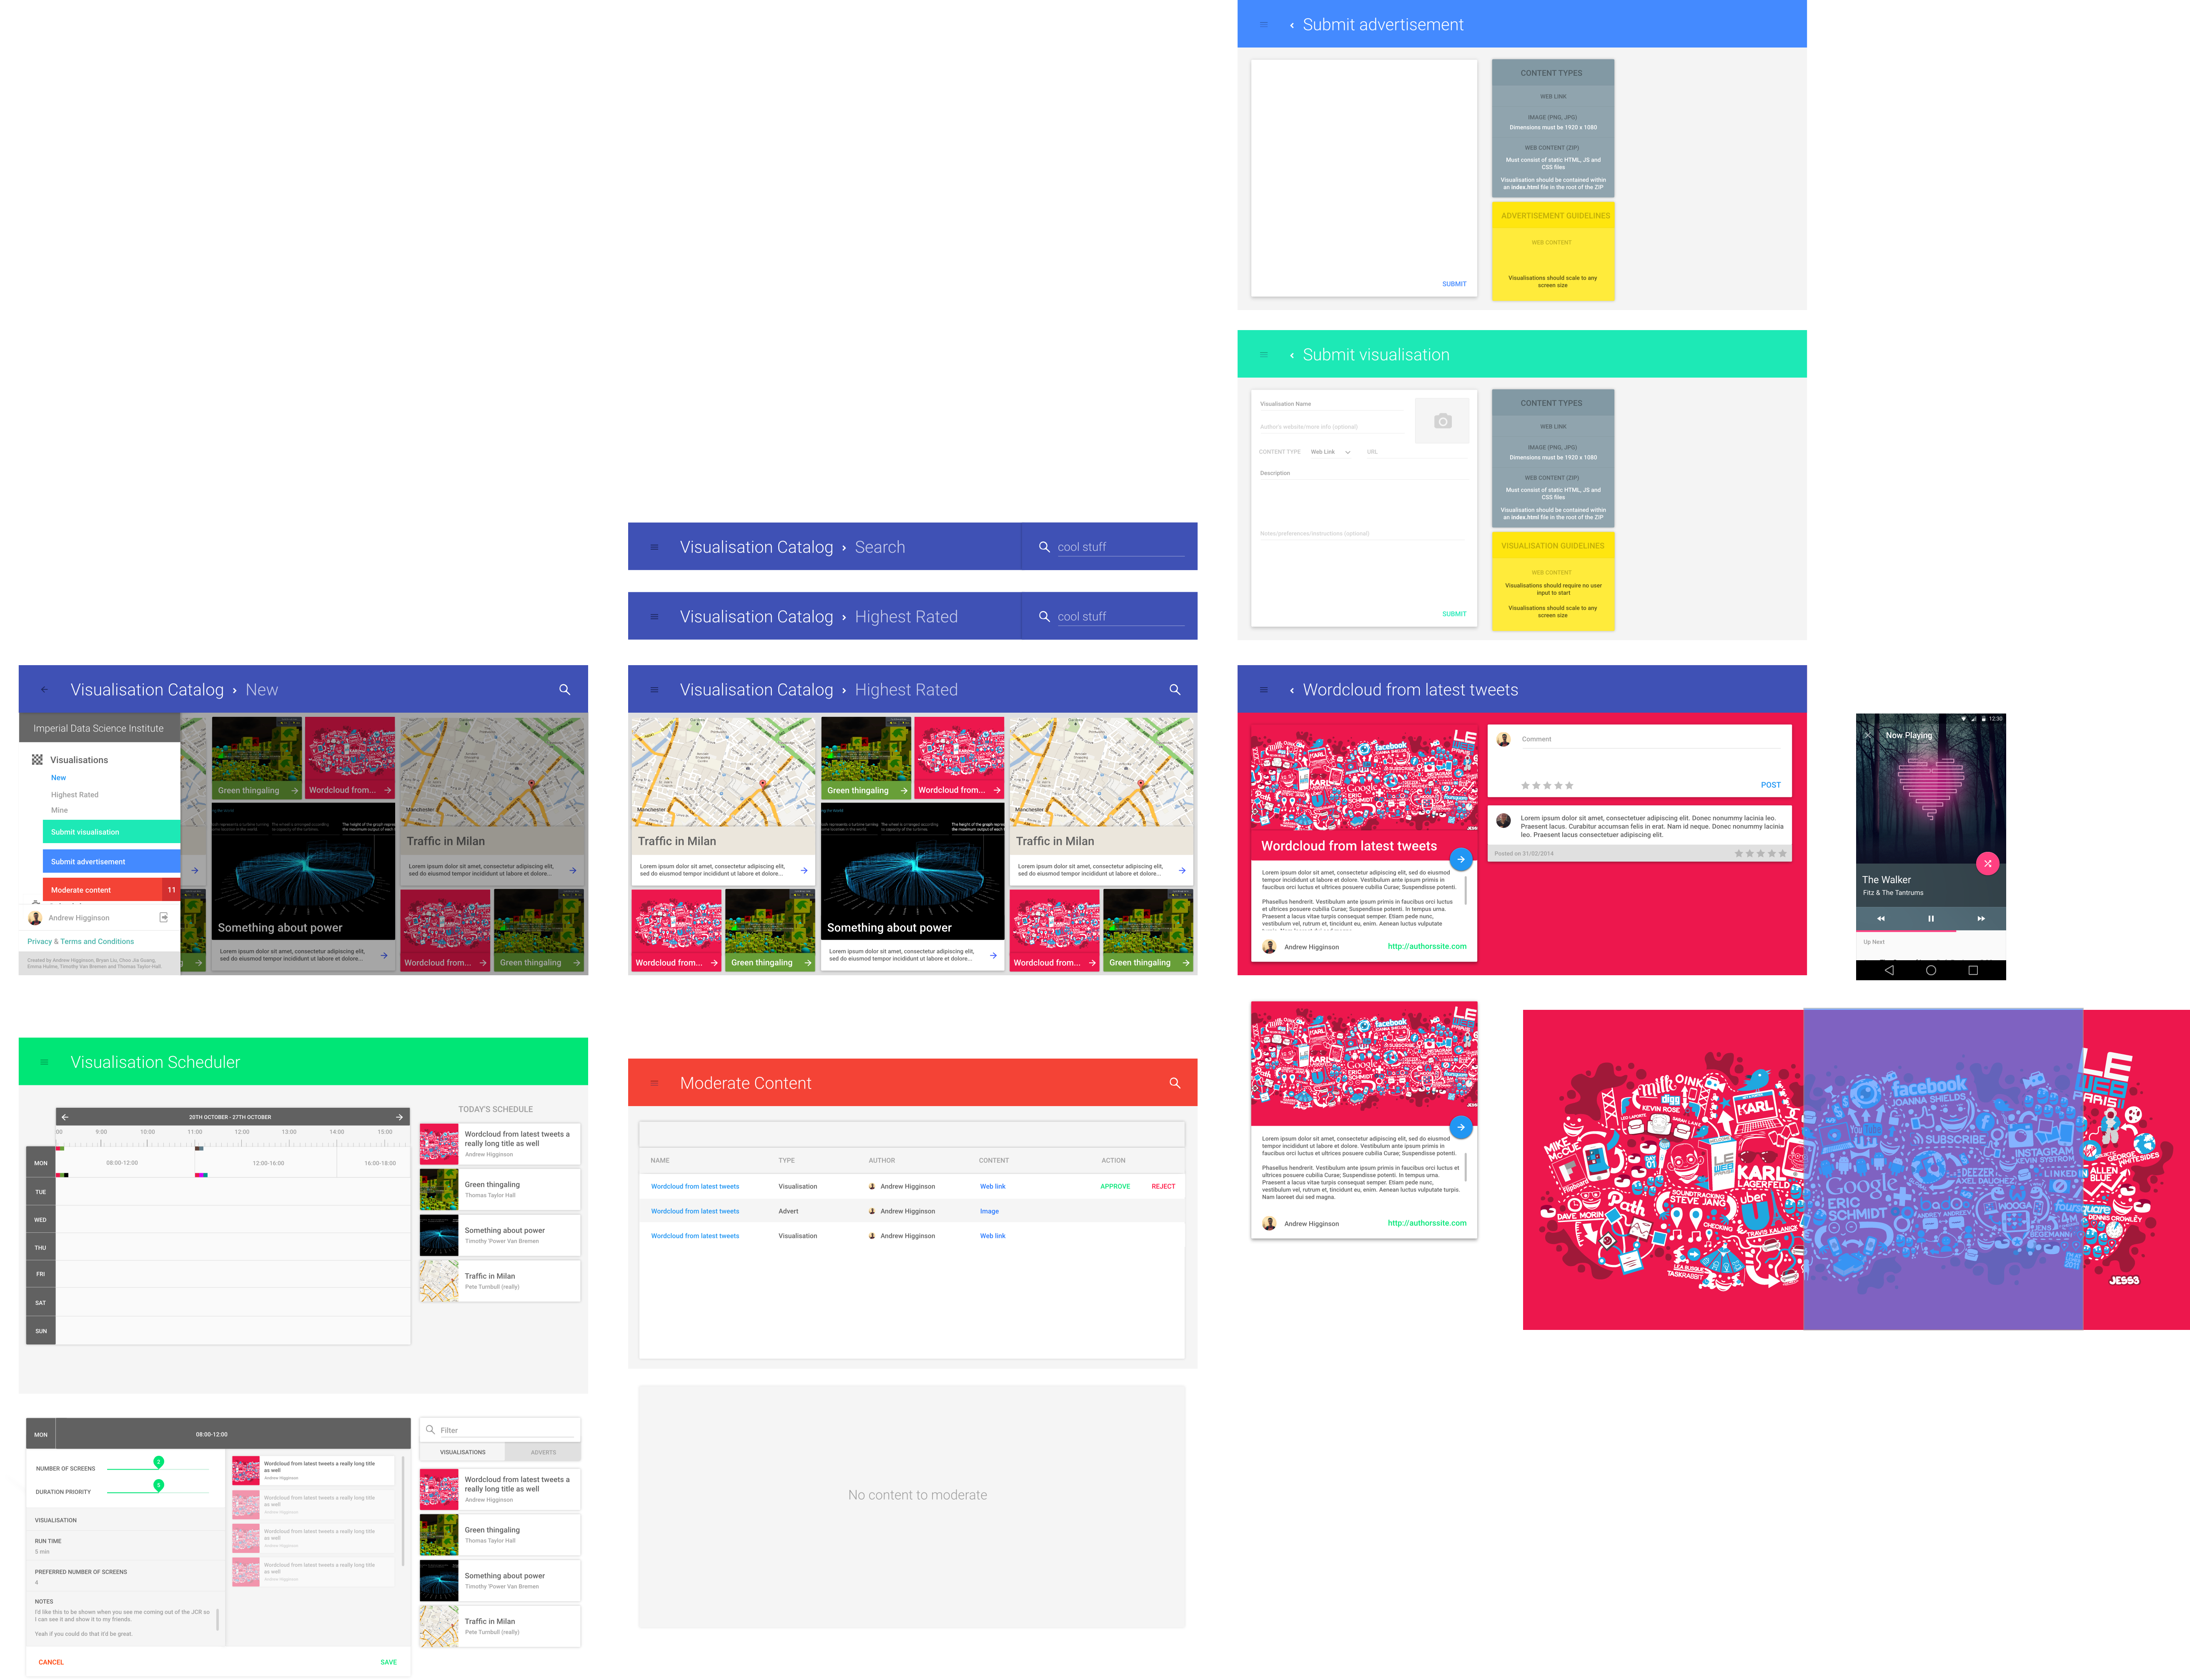
\includegraphics[width = \textwidth]{./evaluation/mockup.png}
   \end{center}
   \caption{Mockups on User Interface}
   \label{fig:mockup}
\end{figure}

\subsection{Scheduling Requirements}
Compared to User Interfaces which user can see and feel, we believe 
uncovering the client's assumption on scheduling via mockups or 
prototypes would not be the most feasible means as it is mainly rule-based.
We instead deliver our ideas with illustrations on whiteboard and
capture feedback from David.

Through discussions with David, we uncovered an assumption that 
the scheduling algorithm should ensure the playout time is 
directly proportional to some metric set by administrators. In response,
we have created additional RSpec unit test to incoperate such requirements 
in our scheduling algorithm.



\begin{figure}[H]
  \begin{minipage}{0.46\textwidth}
      \includegraphics[width = 0.99\textwidth, trim = 0 4.5cm 0 7cm, clip]{./evaluation/scheduling_whiteboard.jpg}
  \end{minipage}
  \begin{minipage}{0.53\textwidth}
      \includegraphics[width = 0.99\textwidth]{./evaluation/scheduling_spec.png}
  \end{minipage}
  \caption{Capturing scheduling requirements on whiteboard (left)\\ and subsequently via RSpec unit tests (right)}
 
\end{figure}


\subsection{Usability Testing}

\section{Evaluation of Project}
%How will we evaluate?
As a group, we are constantly evaluating our project by testing after a 
feature is implemented. We make use of both RSpec and manual testing. In 
addition, our project progress is evaluated by David in our weekly 
meetings. Using Jenkins for Continuous Integration, we have given David
the address of our ``release vm'', where he can see the latest working 
version of the project. From this, David can constantly evaluate our project 
through all stages of development.

Quantitively, we can evaluate our project by ticking off our intial 
requirements. Also, we will use the systems ourselves, both from the user 
and administrator perspective, to evaluate the project from both our stakeholders.
This will include uploading of visualisations and viewing other visualisations as a
user, and moderating and scheduling visualisations as an admin.

Using our Trello board and version control, we can see which features have been 
implemented by which group member. To improve our teamwork for future group 
projects, we will sit down as a group and describe our strengths and weaknesses in 
this project.

TODO: get externals to evaluate, people from data science institute? 

TODO: stuff from eval lecture





\end{document}
